\documentclass[11pt,a4paper]{article}

\usepackage[utf8]{inputenc}
\usepackage[T1]{fontenc}
\usepackage{amsmath,amssymb}
\usepackage{geometry}
\usepackage{booktabs}
\usepackage{listings}
\usepackage{pgfplots}
\usepackage[colorlinks=true,linkcolor=blue,citecolor=blue,urlcolor=blue]{hyperref}

\geometry{left=2.5cm,right=2.5cm,top=2.5cm,bottom=2.5cm}
\pgfplotsset{compat=1.18}

\lstset{
  basicstyle=\ttfamily\small,
  breaklines=true,
  frame=single,
  numbers=left,
  numberstyle=\tiny,
  tabsize=2
}

\title{\textbf{NRR-Coupled (cp) v3: Robust Simulation Evaluation Under Dependency Conditions}}
\author{Kei Saito\\Independent Researcher, Japan\\\texttt{kei.saito.research@gmail.com}}
\date{February 2026\\[0.5em]\textit{Part of the Non-Resolution Reasoning (NRR) research program.}}

\begin{document}
\maketitle

\begin{center}
\textcopyright\ 2026 Kei Saito. Licensed under CC BY 4.0.\\
\url{https://creativecommons.org/licenses/by/4.0/}
\end{center}

\begin{abstract}
NRR-Transfer defines an uncoupled update interface for independent candidates. NRR-Coupled (cp) extends that interface to dependent candidates by adding client-side propagation while preserving LLM-side \((\sigma/\delta,\text{target})\) selection. This version focuses on robust simulation evaluation: instead of a single hand-crafted operator stream, we use 15 seed-fixed random streams for each of three state patterns (\(n=4,5,6\)), totaling 45 runs per condition and coupling level. We compare uncoupled baseline (\(\beta=0\)) and coupled variants (\(\beta\in\{0.1,0.3,0.5\}\)) under dependent, independent, and mismatch matrices. Primary criteria are utility difference and convergence speed (\(\tau\)) against a hidden reference trajectory. At \(\beta=0.3\), cp improves mean utility in dependent condition (+0.0296) and reduces mean convergence turn by 1.53, while mismatch condition degrades mean utility (-0.0453) and slows convergence (+1.47 turns). Independent condition remains exactly equivalent to baseline within tolerance \(10^{-12}\). These results support a conditional claim: coupled propagation is beneficial when dependency structure is correct, and harmful when dependency signs are wrong.
\end{abstract}

\noindent\textbf{Keywords:} NRR-Coupled, dependency propagation, robust simulation, convergence speed, falsifiable evaluation

\section{Introduction}
LLM APIs are stateless across calls, but many systems need iterative state updates over candidate sets. NRR-Transfer addressed independent-candidate updates. This paper addresses dependent-candidate updates through \textbf{NRR-Coupled (cp)}.

NRR is not an anti-LLM framework.
NRR does not replace standard LLM use.
NRR optimizes when to commit and when to defer, under explicit conditions.

\textbf{Claim boundary.}
Transfer: independent candidates.
cp: dependent candidates.
Uncoupled baseline is inherited from Transfer and not redefined here.

\textbf{Fixed interface hypothesis.}
LLM-side decision remains unchanged (\(\sigma/\delta\), target). Only client propagation changes. If this interface breaks, set `TRANSFER\_PRINCIPLES\_REEVAL\_REQUIRED=true` and continue cp-side analysis.

Series Consistency Statement: Unsupported interpretations are never injected at a fixed evidence state. Hypothesis-set expansion is evidence-gated, and unobserved possibilities remain unresolved. Evidence in this paper is restricted to fixed simulation inputs and declared dependency structures.

\section{Coupled Update Rule}
Let \(V=\{1,\dots,n\}\), \(\mathbf{w}_t\in\mathbb{R}^n\), \(\sum_i w_t^{(i)}=1\), and dependency matrix \(A\in\mathbb{R}^{n\times n}\), where \(A_{ij}\) is influence from candidate \(j\) to candidate \(i\).

\subsection{Step 1: local target update (Transfer-compatible)}
\[
\Delta_t = \begin{cases}
+\alpha & (o_t=\sigma),\\
-\alpha & (o_t=\delta),
\end{cases}
\qquad
\tilde{w}^{(k_t)}=\operatorname{clip}(w_t^{(k_t)}+\Delta_t,\varepsilon,u_{\max}).
\]

\subsection{Step 2: coupled propagation (cp extension)}
\[
d_t=\tilde{w}^{(k_t)}-w_t^{(k_t)},\qquad
\tilde{w}^{(i)}\leftarrow\operatorname{clip}(\tilde{w}^{(i)}+\beta A_{i,k_t}d_t,\varepsilon,u_{\max})\;(i\neq k_t).
\]

\subsection{Step 3: Transfer-style renormalization}
Target is fixed; non-targets are proportionally scaled:
\[
w_{t+1}^{(k_t)}=\tilde{w}^{(k_t)},\quad
S_t^- = \sum_{i\neq k_t}\tilde{w}^{(i)},\quad
r_t=1-\tilde{w}^{(k_t)},
\]
\[
w_{t+1}^{(i)}=\frac{\tilde{w}^{(i)}}{S_t^-}r_t\quad(i\neq k_t).
\]
If \(S_t^-=0\), residual mass is uniformly distributed over non-targets.

\subsection{Complexity upper bounds}
For sparse column execution:
\[
T_{\text{turn}}=O\big(n+\deg_{\text{out}}(k_t)\big),
\]
with dense-column worst case \(O(n)\), and naive full-matrix implementation upper bound \(O(n^2)\). Memory is \(O(n+\mathrm{nnz}(A))\) sparse (or \(O(n^2)\) dense).

\section{Robust Simulation Design}
\subsection{Why design changed from single-stream evaluation}
A single hand-crafted stream can hide or exaggerate coupled effects. To test stream-robustness (analogous to Transfer's multi-model robustness), we evaluate many seed-fixed random streams.

\subsection{Patterns and random streams}
Three patterns are used:
\begin{center}
\begin{tabular}{@{}lcc@{}}
\toprule
Pattern & Candidate count & Initial state \\
\midrule
P1-n4 & 4 & $(0.25,0.25,0.25,0.25)$ \\
P2-n5 & 5 & $(0.20,0.20,0.20,0.20,0.20)$ \\
P3-n6 & 6 & uniform \\
\bottomrule
\end{tabular}
\end{center}
For each pattern, 15 operator streams are generated with fixed seeds (\texttt{seed\_base=20260228}), each with 12 turns. Operators are random \((\sigma/\delta,\text{target})\) pairs.

\subsection{Dependency conditions}
Dependent matrices are mixed-sign sparse matrices:
\[
A^{\mathrm{dep}}_{(j+1)\bmod n,j}=p_n,\;
A^{\mathrm{dep}}_{(j+2)\bmod n,j}=q_n<0,\;
A^{\mathrm{dep}}_{(j-1)\bmod n,j}=s_n,
\]
others zero.

Coefficients:
\[
(p_4,q_4,s_4)=(1.20,-0.90,0.70),
\]
\[
(p_5,q_5,s_5)=(1.10,-0.80,0.65),\quad
(p_6,q_6,s_6)=(1.00,-0.75,0.60).
\]

Conditions:
\begin{itemize}
  \item D-dependent: true matrix \(A^{\mathrm{dep}}\), model matrix \(A^{\mathrm{dep}}\)
  \item D-independent: true matrix \(0\), model matrix \(0\)
  \item D-mismatch: true matrix \(A^{\mathrm{dep}}\), model matrix \(-A^{\mathrm{dep}}\)
\end{itemize}

\subsection{Compared systems}
\begin{itemize}
  \item Uncoupled baseline: \(\beta=0\)
  \item Coupled cp: \(\beta\in\{0.1,0.3,0.5\}\)
\end{itemize}
Reference trajectory uses hidden true coupling \(\beta_{\text{true}}=0.5\).

\section{Metrics and Falsifiable Criteria}
Let \(\mathbf{w}^{\mathrm{ref}}_T\) be final reference state after 12 turns.

Distance per turn:
\[
d_t = \lVert \mathbf{w}_t-\mathbf{w}^{\mathrm{ref}}_T \rVert_1.
\]
Utility:
\[
U = 1 - \frac{1}{2T}\sum_{t=1}^{T} d_t,\quad T=12.
\]
Convergence speed:
\[
\tau_{\varepsilon}=\min\{t\mid d_t\le\varepsilon\},\quad \varepsilon=0.25,
\]
(or \(T+1\) if unmet).

Oscillation is sign-flip count in candidate-wise step deltas.
Independent equivalence check:
\[
\max_{t,i}|w^{\mathrm{cp}}_{t,i}-w^{\mathrm{base}}_{t,i}|\le 10^{-12}.
\]

Primary pre-registered checks at \(\beta=0.3\):
\begin{enumerate}
  \item dependent mean \(\Delta\tau=\tau_{cp}-\tau_{base}<0\)
  \item dependent mean \(\Delta U=U_{cp}-U_{base}>0\)
  \item mismatch mean \(\Delta U<0\)
  \item independent mean \(\Delta U\ge 0\) and all equivalence checks pass
\end{enumerate}

\section{Results}
Total paired samples per condition and beta: \(3\) patterns \(\times\) \(15\) streams = \(45\).
Output files: `cp\_v3\_per\_turn.csv`, `cp\_v3\_summary.csv`, `cp\_v3\_pairwise.csv`, `cp\_v3\_aggregate.csv`, `cp\_v3\_independent\_check.csv`, `cp\_v3\_report.json`.

\subsection{Robustness summary (mean $\pm$ sd, with min/max)}
\begin{center}
\begin{tabular}{@{}llcc@{}}
\toprule
Condition & Metric (\(\beta=0.3\)) & Mean $\pm$ SD & Min / Max \\
\midrule
D-dependent & $\Delta U$ & $0.0296 \pm 0.0309$ & $-0.0333 / 0.1184$ \\
D-dependent & $\Delta\tau$ & $-1.5333 \pm 3.1312$ & $-10 / 10$ \\
D-independent & $\Delta U$ & $0.0000 \pm 0.0000$ & $0.0000 / 0.0000$ \\
D-independent & $\Delta\tau$ & $0.0000 \pm 0.0000$ & $0 / 0$ \\
D-mismatch & $\Delta U$ & $-0.0453 \pm 0.0231$ & $-0.0937 / 0.0140$ \\
D-mismatch & $\Delta\tau$ & $1.4667 \pm 2.8253$ & $0 / 11$ \\
\bottomrule
\end{tabular}
\end{center}

\begin{figure}[t]
\centering
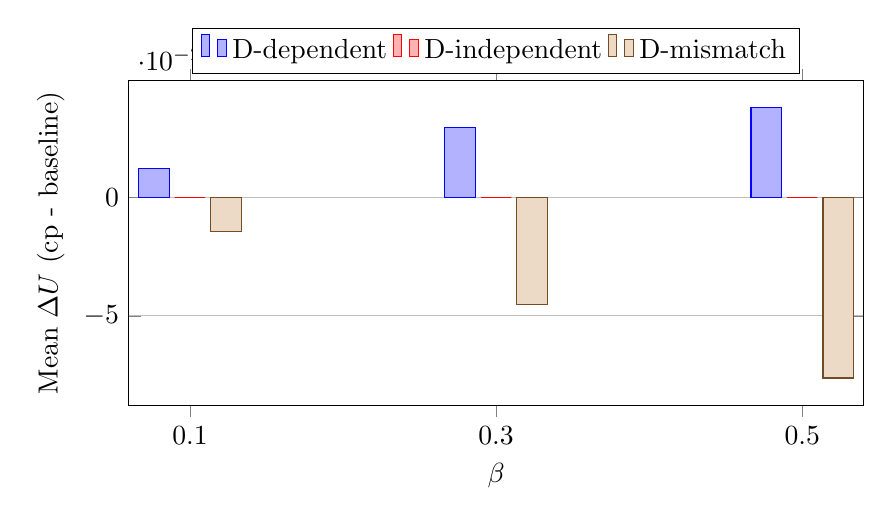
\begin{tikzpicture}
\begin{axis}[
  ybar,
  bar width=11pt,
  width=0.9\textwidth,
  height=5.7cm,
  xlabel={$\beta$},
  ylabel={Mean $\Delta U$ (cp - baseline)},
  symbolic x coords={0.1,0.3,0.5},
  xtick=data,
  legend style={at={(0.5,1.02)},anchor=south,legend columns=3},
  ymajorgrids=true
]
\addplot coordinates {(0.1,0.012343) (0.3,0.029629) (0.5,0.037856)};
\addplot coordinates {(0.1,0.000000) (0.3,0.000000) (0.5,0.000000)};
\addplot coordinates {(0.1,-0.014345) (0.3,-0.045262) (0.5,-0.076217)};
\legend{D-dependent,D-independent,D-mismatch}
\end{axis}
\end{tikzpicture}
\caption{Mean utility difference across 45 samples per condition and beta.}
\label{fig:udiff_v3}
\end{figure}

\begin{figure}[t]
\centering
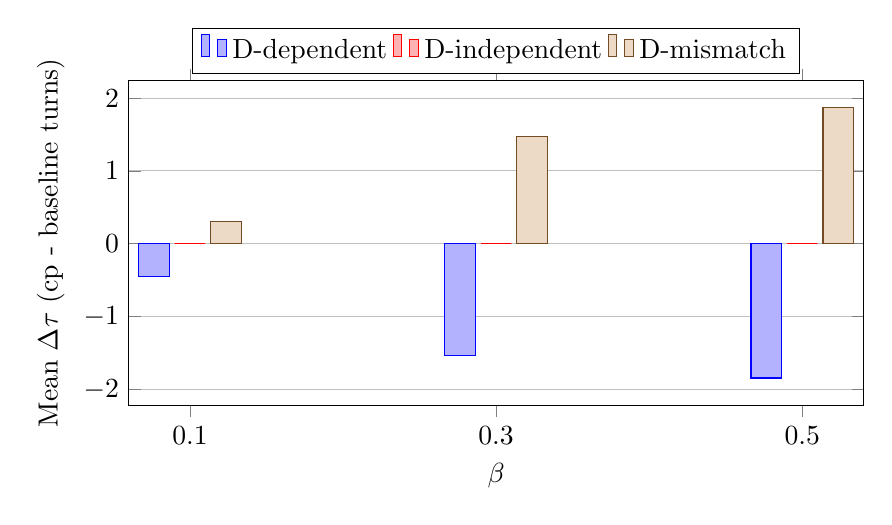
\begin{tikzpicture}
\begin{axis}[
  ybar,
  bar width=11pt,
  width=0.9\textwidth,
  height=5.7cm,
  xlabel={$\beta$},
  ylabel={Mean $\Delta\tau$ (cp - baseline turns)},
  symbolic x coords={0.1,0.3,0.5},
  xtick=data,
  legend style={at={(0.5,1.02)},anchor=south,legend columns=3},
  ymajorgrids=true
]
\addplot coordinates {(0.1,-0.4444) (0.3,-1.5333) (0.5,-1.8444)};
\addplot coordinates {(0.1,0.0000) (0.3,0.0000) (0.5,0.0000)};
\addplot coordinates {(0.1,0.3111) (0.3,1.4667) (0.5,1.8667)};
\legend{D-dependent,D-independent,D-mismatch}
\end{axis}
\end{tikzpicture}
\caption{Mean convergence-turn difference across 45 samples per condition and beta. Negative is faster cp.}
\label{fig:taudiff_v3}
\end{figure}

\subsection{Pass/fail outcomes}
From `cp\_v3\_report.json` (\(\beta=0.3\)):
\begin{itemize}
  \item dependent tau gain: pass
  \item dependent utility gain: pass
  \item mismatch penalty: pass
  \item independent non-regression: pass
  \item independent equivalence (tol \(10^{-12}\)): pass
\end{itemize}

\section{Applicability and Failure Conditions}
Applicable when dependency matrix quality is sufficient and coupling is bounded.

Failure modes:
\begin{enumerate}
  \item wrong-sign dependency matrix causing degradation (observed in D-mismatch),
  \item over-coupling instability/oscillation,
  \item parse failure of \((\sigma/\delta,\text{target})\) interface.
\end{enumerate}
For parse/interface failure, set `TRANSFER\_PRINCIPLES\_REEVAL\_REQUIRED=true`.

\section{Reproducibility}
Artifacts:
\begin{itemize}
  \item `spec/nrr-coupled\_spec\_v3.md`
  \item `repro/coupled\_state\_sim.py`
  \item `repro/README\_v3.md`
\end{itemize}

Main run command:
\begin{lstlisting}
python3 repro/coupled_state_sim.py --outdir repro/results
\end{lstlisting}

\section{Conclusion}
With stream-robust simulation, cp shows consistent conditional behavior: improvements in dependent settings, exact equivalence under independence, and clear degradation under mismatch. This resolves the single-stream ambiguity and strengthens falsifiability of the cp claim boundary.

\begin{thebibliography}{9}
\bibitem{saito2025nrr}
Saito, K. (2025).
\textit{NRR-Core: Non-Resolution Reasoning as a Computational Framework for Contextual Identity and Ambiguity Preservation}.
arXiv:2512.13478.

\bibitem{saito2026phi}
Saito, K. (2026).
\textit{NRR-Phi: Text-to-State Mapping for Ambiguity Preservation in LLM Inference}.
arXiv:2601.19933.

\bibitem{saito2026transfer}
Saito, K. (2026).
\textit{NRR-Transfer: Cross-Domain Transfer of Phase 1.5 Operators Under Fixed Interface Constraints}.
Manuscript v30 (pre-submission line).
\end{thebibliography}

\end{document}
